\chapter{Including PDFs}\label{sec:includingpdfs}
	\note{The PDFs are inserted at 85\% their full size to ensure that they don't overlap any GPS page formatting required for the headers and footers.}
	
	\warning{While it is possible to have horizontal pages have the page numbers centered on the bottom long edge, I \textit{DO NOT} recommended it. This is because, while it looks okay in a digital format, this is not suitable for printing... this would print page numbers on the side of the page rather than consistently on the bottom.}
	
	\section{How to Insert a Portrait PDF}
		To insert a portrait-oriented PDF into your LaTeX document, you can use the \texttt{pdfpages} package, which provides a convenient way to include external PDF files. 
		The following code snippet demonstrates how to include a portrait PDF with the specified options:
		
		\begin{lstlisting}[float=ht,caption=,label=lst:portraitPDF,style=LaTeXStyle,basicstyle=\ttfamily,]

\includepdf[landscape=false,pages=-,pagecommand={},scale=0.85]{./99_Inclusions/PDFs/examplePDF}
		\end{lstlisting}
		
		In this example, \lstinline|landscape=false| ensures that the PDF is inserted in portrait mode, \lstinline|pages=-| includes all pages of the PDF, \lstinline|pagecommand={}| avoids adding any additional LaTeX commands to each page, and \lstinline|scale=0.85| scales the PDF to 85\% of its original size. 
		Adjust these options as needed for your document.
		
		
\includepdf[landscape=false,pages=-,pagecommand={},scale=0.85]{./99_Inclusions/PDFs/examplePDF}
	\section{How to Insert a Landscape PDF}
		Inserting a landscape-oriented PDF is similarly straightforward using the \texttt{pdfpages} package. 
		The code snippet below demonstrates how to include a landscape PDF:
		
		\begin{lstlisting}[float=ht,caption=,label=lst:landscapePDF,style=LaTeXStyle,basicstyle=\ttfamily,]
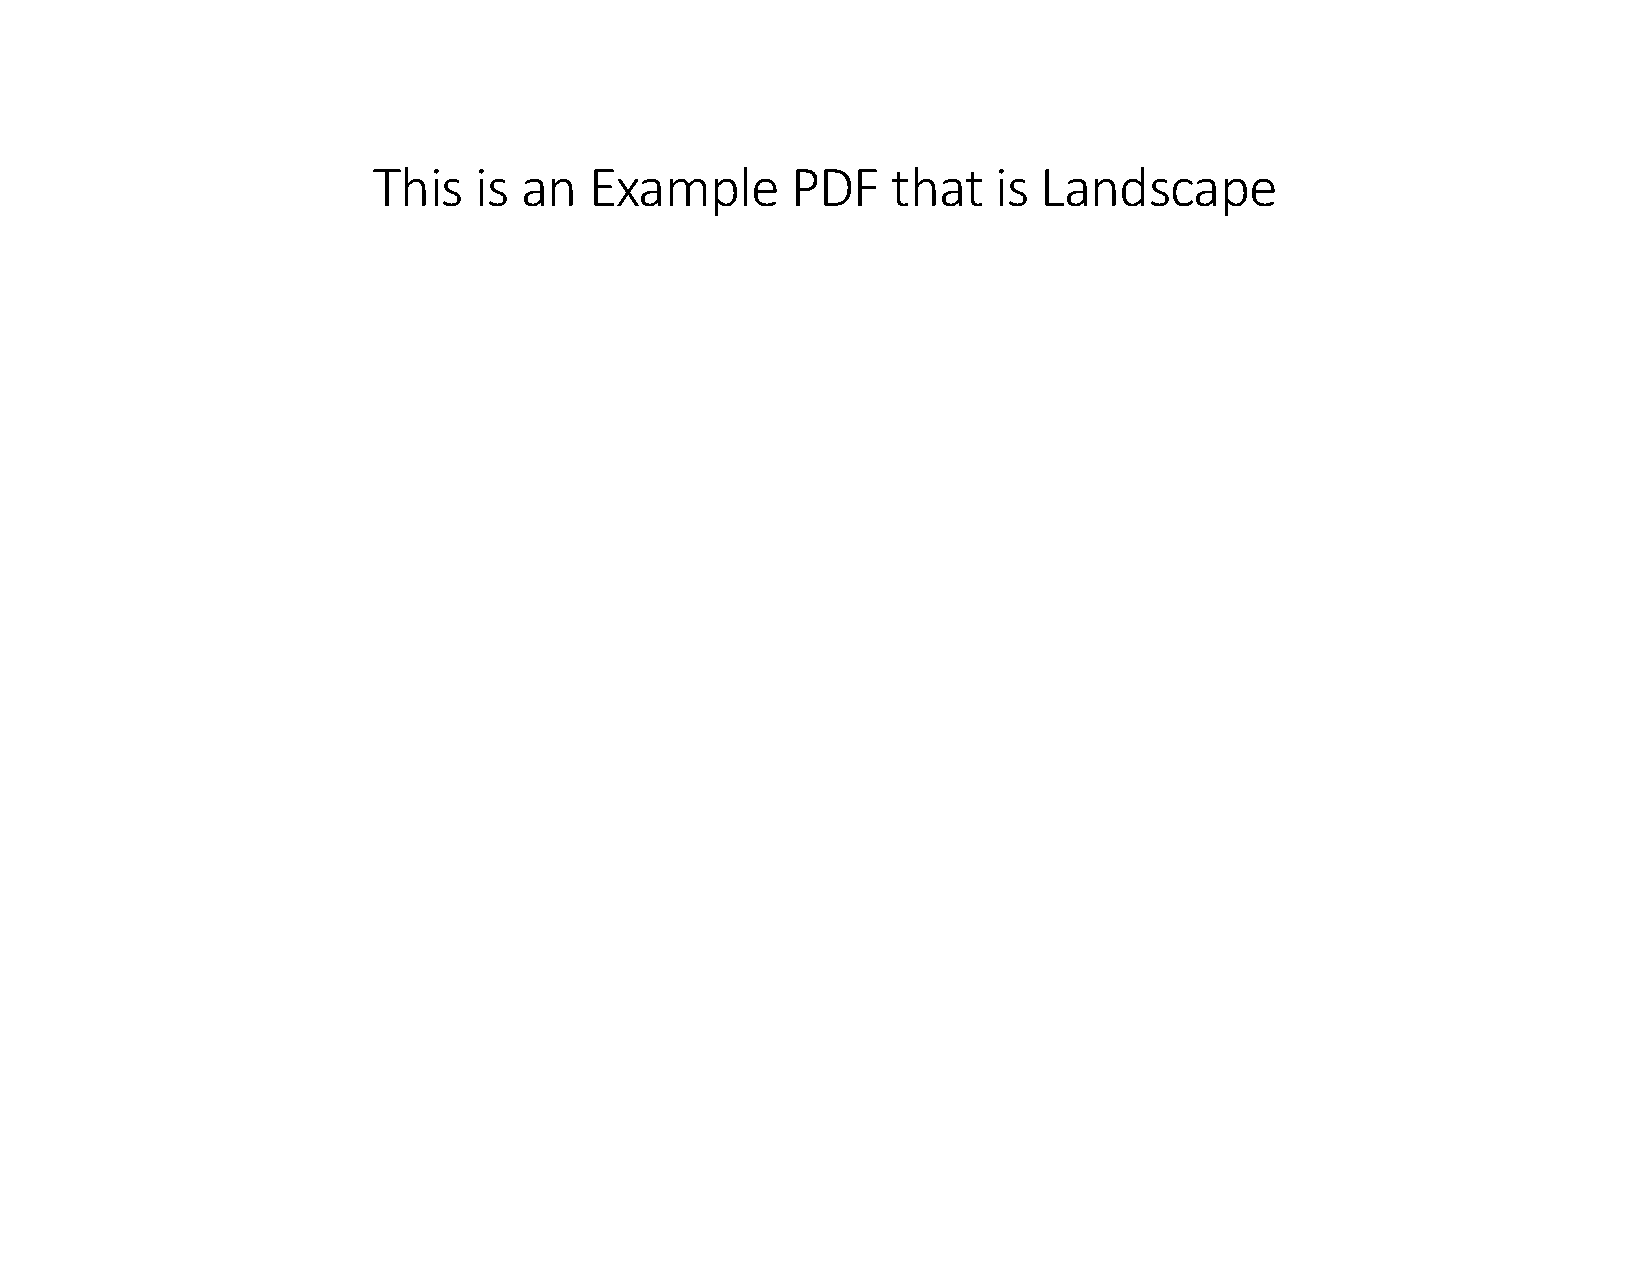
\includepdf[landscape=true,pages=-,pagecommand={},scale=0.85]{./99_Inclusions/PDFs/landscapePDF}
		\end{lstlisting}
		
		Here, \lstinline|landscape=true| sets the orientation to landscape, \lstinline|pages=-| includes all pages from the PDF, \lstinline|pagecommand={}| prevents any extra LaTeX commands on each page, and \lstinline|scale=0.85| scales the inserted PDF to 85\% of its original size. 
		This configuration ensures that your landscape PDF is correctly oriented and properly sized within your document.
		
		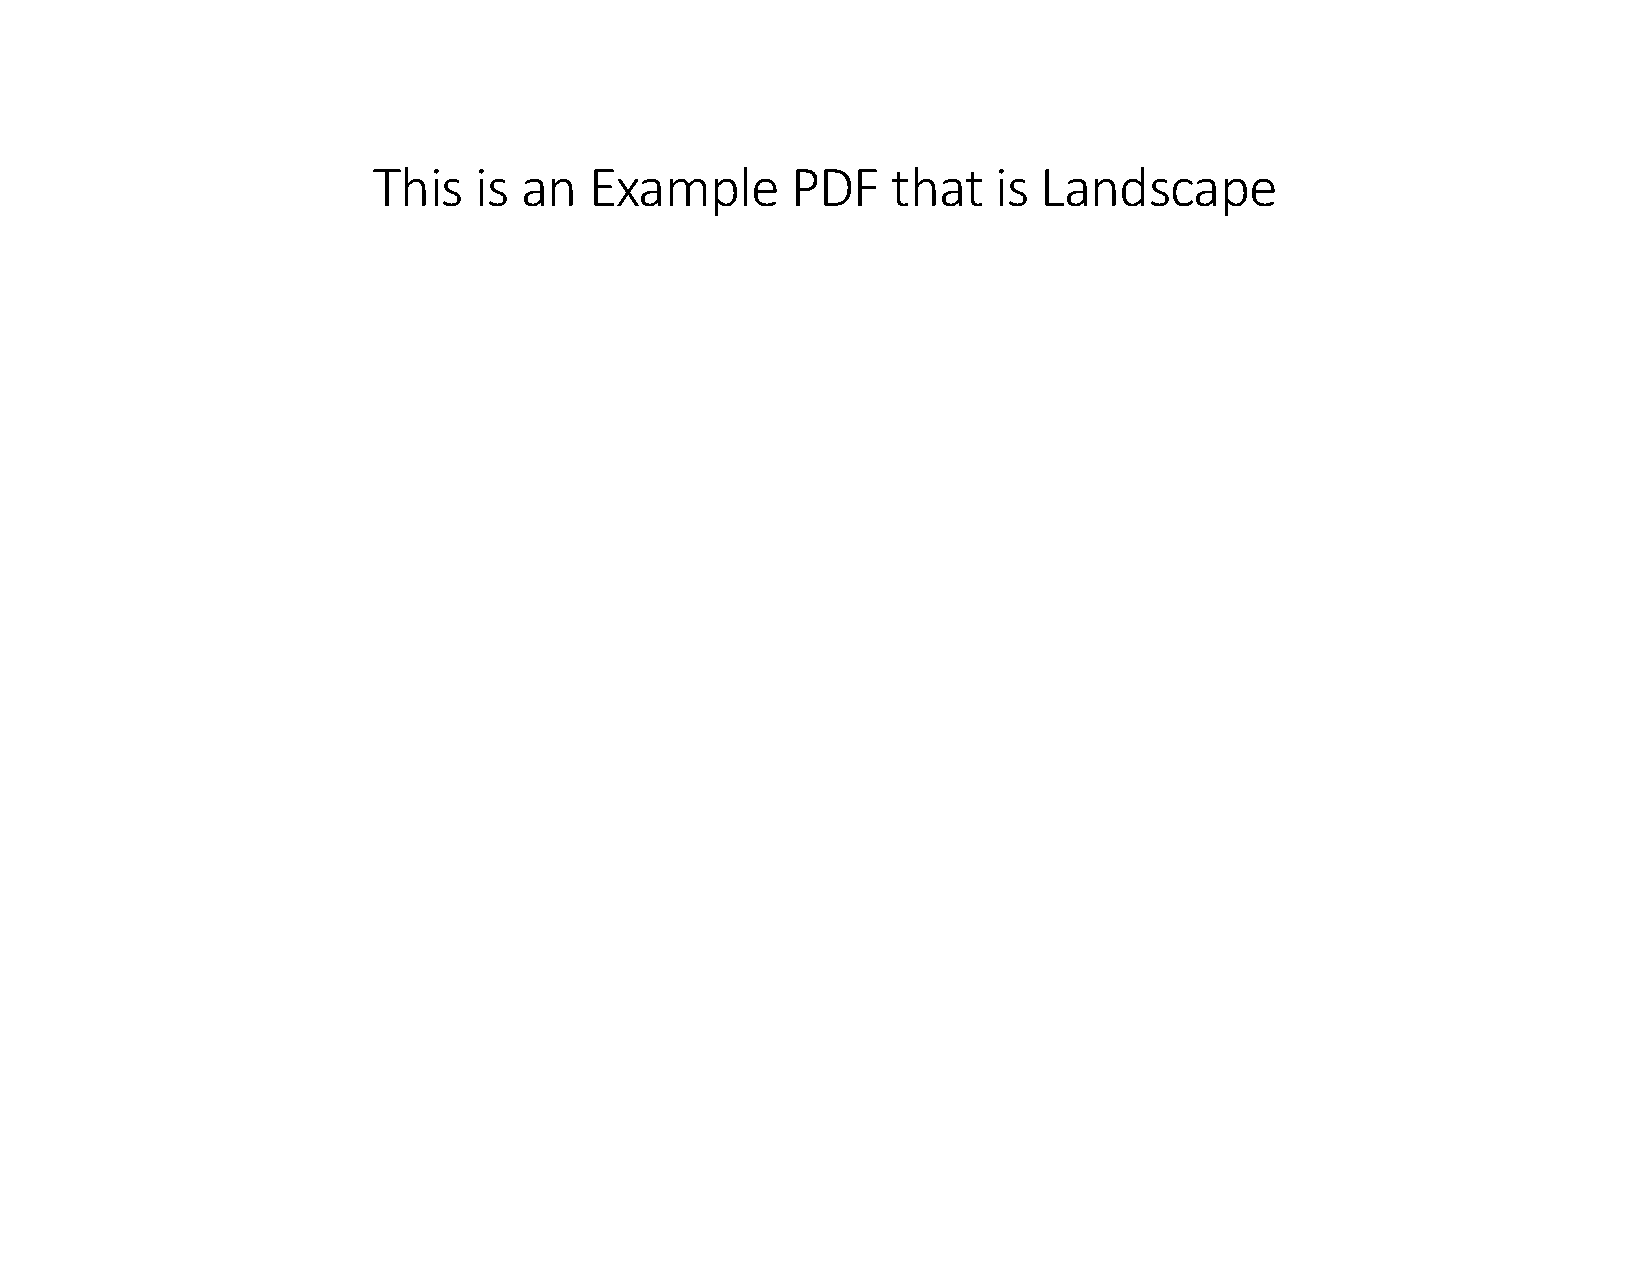
\includepdf[landscape=true,pages=-,pagecommand={},scale=0.85]{./99_Inclusions/PDFs/landscapePDF}